% Options for packages loaded elsewhere
\PassOptionsToPackage{unicode}{hyperref}
\PassOptionsToPackage{hyphens}{url}
\documentclass[
  ignorenonframetext,
]{beamer}
\newif\ifbibliography
\usepackage{pgfpages}
\setbeamertemplate{caption}[numbered]
\setbeamertemplate{caption label separator}{: }
\setbeamercolor{caption name}{fg=normal text.fg}
\beamertemplatenavigationsymbolsempty
% remove section numbering
\setbeamertemplate{part page}{
  \centering
  \begin{beamercolorbox}[sep=16pt,center]{part title}
    \usebeamerfont{part title}\insertpart\par
  \end{beamercolorbox}
}
\setbeamertemplate{section page}{
  \centering
  \begin{beamercolorbox}[sep=12pt,center]{section title}
    \usebeamerfont{section title}\insertsection\par
  \end{beamercolorbox}
}
\setbeamertemplate{subsection page}{
  \centering
  \begin{beamercolorbox}[sep=8pt,center]{subsection title}
    \usebeamerfont{subsection title}\insertsubsection\par
  \end{beamercolorbox}
}
% Prevent slide breaks in the middle of a paragraph
\widowpenalties 1 10000
\raggedbottom
\AtBeginPart{
  \frame{\partpage}
}
\AtBeginSection{
  \ifbibliography
  \else
    \frame{\sectionpage}
  \fi
}
\AtBeginSubsection{
  \frame{\subsectionpage}
}
\usepackage{iftex}
\ifPDFTeX
  \usepackage[T1]{fontenc}
  \usepackage[utf8]{inputenc}
  \usepackage{textcomp} % provide euro and other symbols
\else % if luatex or xetex
  \usepackage{unicode-math} % this also loads fontspec
  \defaultfontfeatures{Scale=MatchLowercase}
  \defaultfontfeatures[\rmfamily]{Ligatures=TeX,Scale=1}
\fi
\usepackage{lmodern}
\ifPDFTeX\else
  % xetex/luatex font selection
\fi
% Use upquote if available, for straight quotes in verbatim environments
\IfFileExists{upquote.sty}{\usepackage{upquote}}{}
\IfFileExists{microtype.sty}{% use microtype if available
  \usepackage[]{microtype}
  \UseMicrotypeSet[protrusion]{basicmath} % disable protrusion for tt fonts
}{}
\makeatletter
\@ifundefined{KOMAClassName}{% if non-KOMA class
  \IfFileExists{parskip.sty}{%
    \usepackage{parskip}
  }{% else
    \setlength{\parindent}{0pt}
    \setlength{\parskip}{6pt plus 2pt minus 1pt}}
}{% if KOMA class
  \KOMAoptions{parskip=half}}
\makeatother
\usepackage{longtable,booktabs,array}
\newcounter{none} % for unnumbered tables
\usepackage{calc} % for calculating minipage widths
\usepackage{caption}
% Make caption package work with longtable
\makeatletter
\def\fnum@table{\tablename~\thetable}
\makeatother
\usepackage{graphicx}
\makeatletter
\newsavebox\pandoc@box
\newcommand*\pandocbounded[1]{% scales image to fit in text height/width
  \sbox\pandoc@box{#1}%
  \Gscale@div\@tempa{\textheight}{\dimexpr\ht\pandoc@box+\dp\pandoc@box\relax}%
  \Gscale@div\@tempb{\linewidth}{\wd\pandoc@box}%
  \ifdim\@tempb\p@<\@tempa\p@\let\@tempa\@tempb\fi% select the smaller of both
  \ifdim\@tempa\p@<\p@\scalebox{\@tempa}{\usebox\pandoc@box}%
  \else\usebox{\pandoc@box}%
  \fi%
}
% Set default figure placement to htbp
\def\fps@figure{htbp}
\makeatother
\setlength{\emergencystretch}{3em} % prevent overfull lines
\providecommand{\tightlist}{%
  \setlength{\itemsep}{0pt}\setlength{\parskip}{0pt}}
% Auto-generated by infrastructure/rendering/_pdf_latex_helpers.py::extract_math_font_preamble.
% Minimal header passed to Pandoc via -H so Beamer slides pick up the same math font
% as the combined-PDF path. Adjust the manuscript's preamble.md to change the font globally.
\usepackage{unicode-math}
\setmathfont{latinmodern-math.otf}

% Slide layout defaults for warning-clean scientific decks.
\usepackage{etoolbox}
\IfFileExists{xurl.sty}{\usepackage{xurl}}{}
\IfFileExists{seqsplit.sty}{\usepackage{seqsplit}}{\newcommand{\seqsplit}[1]{#1}}
\protected\def\breakseq#1{\seqsplit{#1}}
\protected\def\breaktt#1{\begingroup\ttfamily\seqsplit{#1}\endgroup}
\setlength{\emergencystretch}{6em}
\tolerance=5000
\hbadness=10000
\hfuzz=1pt
\setlength{\tabcolsep}{2pt}
\AtBeginEnvironment{longtable}{\tiny\renewcommand{\arraystretch}{0.86}\setlength{\tabcolsep}{1pt}}
\AtBeginEnvironment{tabular}{\tiny\renewcommand{\arraystretch}{0.86}\setlength{\tabcolsep}{1pt}}

% Natbib and cross-reference fallbacks — slides don't load natbib
% or cleveref, but combined-PDF manuscript prose may emit these
% commands. The fallback renders citations as a bracketed key list
% and cross-references as detokenized labels so slides don't fail on
% undefined control sequences or raw underscores. \providecommand is
% a no-op if packages load later.
\providecommand{\citep}[1]{[#1]}
\providecommand{\citet}[1]{#1}
\providecommand{\citealp}[1]{#1}
\providecommand{\citeauthor}[1]{#1}
\providecommand{\citeyear}[1]{#1}
\providecommand{\cref}[1]{\texttt{\detokenize{#1}}}
\providecommand{\Cref}[1]{\texttt{\detokenize{#1}}}
\usepackage{bookmark}
\IfFileExists{xurl.sty}{\usepackage{xurl}}{} % add URL line breaks if available
\urlstyle{same}
% fallback for those not using the hyperref driver hyperxmp:
\makeatletter
\@ifundefined{xmpquote}{\newcommand{\xmpquote}[1]{#1}}{}
\makeatother
\hypersetup{
  hidelinks,
  pdfcreator={LaTeX via pandoc}}

\author{\texorpdfstring{}{}}
\date{}

\begin{document}

\section{Results}\label{sec:results}

\begin{frame}[fragile,allowframebreaks]{Results}
This section reports the compiled plans for both worked example methods.
Every number below is produced by the thin analysis script
(\href{https://github.com/docxology/template/blob/main/projects/templates/template_methods_paper/scripts/methods_analysis.py}{\breaktt{scripts/methods\_analysis.py}}),
which calls \texttt{run\_all\_gates} and \texttt{compile\_method} from
\breaktt{src/methods\_dsl/} and writes
\breaktt{output/data/compiled\_plans.json},
\breaktt{output/reports/gate\_report.json}, and
\breaktt{output/reports/trust\_chain\_report.json}. Running the script
regenerates every artifact this section references.
\end{frame}

\begin{frame}[fragile,allowframebreaks]{Compiled-plan summary}
\protect\phantomsection\label{compiled-plan-summary}
\begin{longtable}[]{@{}llll@{}}
\caption{Compiled-plan summary from
\protect\breaktt{output/data/compiled\_plans.json}, generated by
\protect\texttt{compile\_method} for each of 2 worked example
methods.}\label{tbl:compiled_plans}\tabularnewline
\toprule\noalign{}
Method & Steps & Target & Plan hash (first 12 hex chars) \\
\midrule\noalign{}
\endfirsthead
\toprule\noalign{}
Method & Steps & Target & Plan hash (first 12 hex chars) \\
\midrule\noalign{}
\endhead
\texttt{PBSPreparation} & 5 & \texttt{human} & \texttt{313b9b17de98} \\
\breaktt{SensorCalibrationSweep} & 4 & \texttt{automated} &
\texttt{d89cced19be6} \\
\bottomrule\noalign{}
\end{longtable}

\breakseq{[@tbl:compiled\_plans]} shows \texttt{PBSPreparation} (a manual,
\texttt{HUMAN}-target bench preparation) alongside
\breaktt{SensorCalibrationSweep} (a mixed
\texttt{AUTOMATED}/\texttt{HUMAN} instrument-calibration procedure) ---
the second example exists specifically to demonstrate the controlled
vocabulary generalizing beyond wet-lab protocols, as
\breakseq{[@sec:introduction]} claims.
\end{frame}

\begin{frame}[fragile,allowframebreaks]{Step-count comparison}
\protect\phantomsection\label{step-count-comparison}
\breakseq{[@fig:step\_counts]} plots the step count for each compiled method.

\begin{figure}
\centering
\pandocbounded{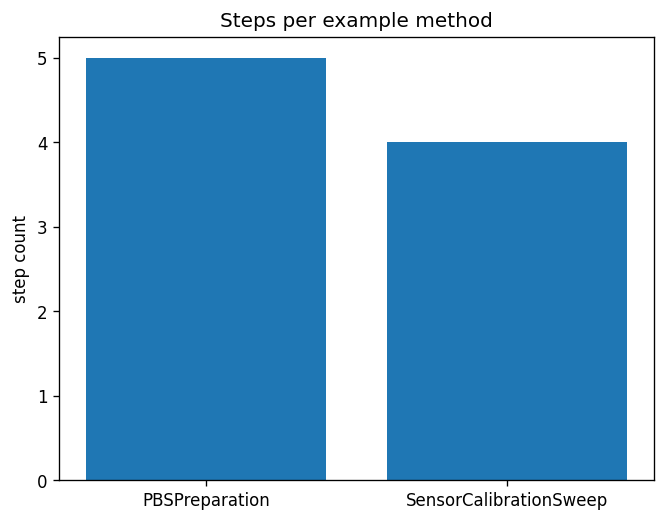
\includegraphics[keepaspectratio,alt={Steps per example method: a bar chart built from len(plan.steps) for each plan in output/data/compiled\_plans.json, plotted by scripts/methods\_analysis.py.}]{../figures/step_counts.png}}
\caption{Steps per example method: a bar chart built from
\protect\texttt{len(plan.steps)} for each plan in
\protect\breaktt{output/data/compiled\_plans.json}, plotted by
\protect\breaktt{scripts/methods\_analysis.py}.}\label{fig:step_counts}
\end{figure}
\end{frame}

\begin{frame}[fragile,allowframebreaks]{Validation gates}
\protect\phantomsection\label{validation-gates}
Across both methods, the analysis script tallies 8 of 8 staged-gate
evaluations passing (\texttt{run\_all\_gates} × 2 methods × 4 gates
each). Every gate result is written to
\breaktt{output/reports/gate\_report.json} --- neither method in this
manuscript is hand-picked to pass; both worked examples are constructed
to satisfy the structural, semantic, plan, and target gates by design,
since \texttt{compile\_method} raises \breaktt{MethodValidationError} and
halts the pipeline on any gate failure.
\end{frame}

\begin{frame}[fragile,allowframebreaks]{Determinism}
\protect\phantomsection\label{determinism}
Recompiling each example method twice and comparing \texttt{plan\_hash}
values yields: \textbf{determinism check = Yes}. This is a live
re-compilation comparison performed by
\breaktt{src/manuscript\_variables.py} at manuscript-build time, not a
value asserted once and then transcribed --- the same property
\breakseq{[@sec:methodology]} claims for \texttt{compile\_method} is checked
again here, independently, against the live build.
\end{frame}

\begin{frame}[fragile,allowframebreaks]{Provenance demonstration}
\protect\phantomsection\label{provenance-demonstration}
\breaktt{scripts/methods\_analysis.py} appends a 3-record demonstration
hash-chain for one value (\breaktt{calibration\_offset}) through
\texttt{DECLARED} → \texttt{CALIBRATED} → \texttt{VERIFIED} tiers and
writes the result of \texttt{verify\_chain} to
\breaktt{output/reports/trust\_chain\_report.json}: \textbf{chain
verified = Yes}.
\end{frame}

\begin{frame}[fragile,allowframebreaks]{Validation}
\protect\phantomsection\label{validation}
The results were validated through the zero-mock \texttt{tests/} suite:

\begin{itemize}
\tightlist
\item
  \textbf{Library tests} assert exact gate outcomes, scheduling order,
  and plan-hash determinism against real \texttt{Method} fixtures,
  including one fixture per gate-failure mode.
\item
  \textbf{Script test} runs \breaktt{run\_methods\_analysis()} against a
  temporary output root and confirms real worklist/CSV/Mermaid/JSON
  artifacts, reports, and a real PNG figure are written.
\item
  \textbf{Manuscript-variable test} confirms every generated-variable
  name used in \texttt{manuscript/*.md} is emitted by
  \breaktt{generate\_variables}.
\end{itemize}

All tests pass with coverage exceeding the 90\% project gate, with no
mocks.
\end{frame}

\begin{frame}[fragile,allowframebreaks]{Discussion}
\protect\phantomsection\label{discussion}
The results confirm the pipeline end to end: both worked examples pass
every staged gate, compile deterministically, and produce a stable plan
hash across repeated builds. The same \breaktt{src/methods\_dsl/}
functions back the analysis script, the test suite, and this manuscript
--- which is the architectural point of the exemplar. Because every
number here is produced by a tested function and regenerated on demand,
the prose describes structure and provenance rather than transcribing
values that would drift the moment the example methods changed.
\end{frame}

\end{document}
